\section{Analysis}

To be included in this section
\begin{enumerate}
    \item ablation: number of training loops
    \item (?) ablation: PPO training on real env
    \item model measures (next frame accuracy, long term value prediction) don't determine final RL performance - how well we can justify it?
    \item  shared weights WM/P models
    \item effects of limited horizon -- e.g. pong/pacman doesn't restart, montezuma dies when jumping in place;
    bank heist story why stochastic model is better - not true?
    \item using of random starts is essential (?)
\end{enumerate}

\todo[inline]{All text in this section is just a placeholder; for mode details see the doc}
\label{envs}
\label{sec:envs}
% \todo[inline]{Here we describe interesting environments; this was quite nicely done in Chiappa's work as well as in Oh's work and this is the place where we want to discuss BankHeist}
In this section we describe \pong, \breakout\ and \freeway\ environments. These environments were introduced in the Arcade Learning Environment (ALE) \cite{ale} (see also \cite{ale2} for a current overview of challenges and successes of various learning methods in ALE). 

\paragraph{Dimensions of input and output.} The screen as given by the ALE emulator consists of an RGB image of the size $160\times 210$ pixels\todo[inline]{Is it rally true?}.  The action space consists of up to 18 actions\todo[inline]{MB.1.16: this is game dependent}. The reward in all games is an integer number\todo[inline]{MB.1.16: which we truncate to -1 0 and 1}.

\paragraph{\pong.} In \pong\ the player is expected to move the green paddle. The red paddle is operated by the original game AI. If the ball crosses the left end of the screen, then the green player scores a point. If the ball crosses the right end of the screen, then the red player scores a point. The total reward for the game is the difference between points scored by the green player and the red player. A full episode lasts until one of the agents scores 21 points. An environment for \pong\ was trained in \cite{recurrent}. Authors reported occasional disappearance of the ball and blurriness of paddles. In order to simplify learning of the environment we considered a modified environment with a ball of the size $10\times 10$ pixels. The change concerns only the observation and not rules of the game. 

\begin{figure}[H]
\makebox[\columnwidth]{%
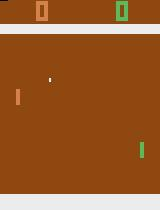
\includegraphics[width=0.24\columnwidth]{figures/PongDeterministic-v4__0}%
\hfill    
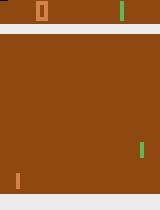
\includegraphics[width=0.24\columnwidth]{figures/PongDeterministic-v4__3.jpg}%
\hfill
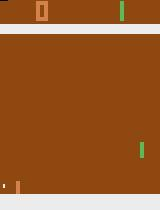
\includegraphics[width=0.24\columnwidth]{figures/PongDeterministic-v4__9.jpg}%
\hfill    
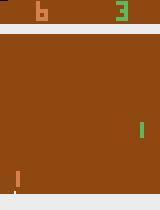
\includegraphics[width=0.24\columnwidth]{figures/PongDeterministic-v4__31.jpg}%
}%
\caption{Four frames from the \pong\ environment. }
\label{fig:pong_original}
\end{figure}


\paragraph{\breakout.} In \breakout\ the player is expected to move the paddle located at the bottom of the screen. The paddle can be moved in the and right directions to the end of the screen. When the ball hits the wall of the bricks, points are scored depending on the color of the brick. The player has 5 lives and the beginning of the game. A life is lost whenever the ball crosses the bottom of the screen.  The environment makes appearance in \cite{recurrent} and is considered as a difficult environment to model, see page 18 of \cite{recurrent}. As in the case of \pong\ in the modified environment we allowed for a ball of the size $10\times 10$ pixels.

% \begin{comment}
\begin{figure}[H]
\makebox[\columnwidth]{%
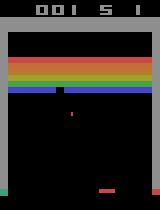
\includegraphics[width=0.24\columnwidth]{figures/BreakoutDeterministic-v4__0}%
\hfill    

\includegraphics[width=0.24\columnwidth]{figures/BreakoutDeterministic-v4__2.jpg}%
\hfill
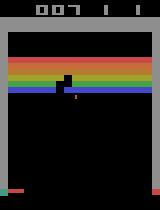
\includegraphics[width=0.24\columnwidth]{figures/BreakoutDeterministic-v4__3.jpg}%
\hfill    

\includegraphics[width=0.24\columnwidth]{figures/BreakoutDeterministic-v4__6.jpg}%
}%
\caption{Four frames from the original \breakout\ environment. }
\label{fig:breakout_original}
\end{figure}
% \end{comment}

\begin{comment}
\begin{figure}[H]
\makebox[\columnwidth]{%

\includegraphics[width=0.24\columnwidth]{figures_mod/BreakoutDeterministic-v4__0}%
\hfill    
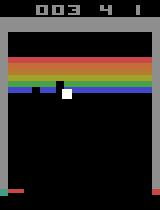
\includegraphics[width=0.24\columnwidth]{figures_mod/BreakoutDeterministic-v4__1.jpg}%
\hfill

\includegraphics[width=0.24\columnwidth]{figures_mod/BreakoutDeterministic-v4__2.jpg}%
\hfill    

\includegraphics[width=0.24\columnwidth]{figures_mod/BreakoutDeterministic-v4__4.jpg}%
}%
\caption{Four frames from the modified \breakout\ environment. }
\label{fig:breakout_mod}
\end{figure}
\end{comment}

\paragraph{\freeway.} In \freeway\ the player is expected to move the yellow chicken from the bottom of the screen to the top of the screen.  The chicken moves only vertically. A point is obtained in the game if the chicken reaches the top of the screen. There is no concept of life, but if the chicken is hit by a car, then it falls approximately 2 lanes down. The environment makes appearance in \cite{recurrent} and is considered as an easy environment to model \cite[page 18]{recurrent} frames. The problem though are the sparse rewards, since the only time a non-0 reward occurs is at the top of the screen.  

%\begin{comment}
\begin{figure}[H]
\makebox[\columnwidth]{%
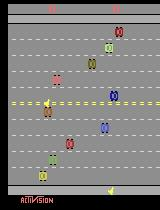
\includegraphics[width=0.24\columnwidth]{figures/FreewayDeterministic-v4__0}%
\hfill    
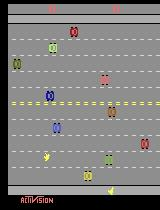
\includegraphics[width=0.24\columnwidth]{figures/FreewayDeterministic-v4__4.jpg}%
\hfill
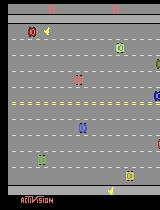
\includegraphics[width=0.24\columnwidth]{figures/FreewayDeterministic-v4__6.jpg}%
\hfill    
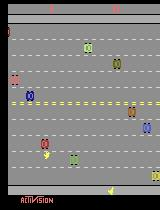
\includegraphics[width=0.24\columnwidth]{figures/FreewayDeterministic-v4__8.jpg}%
}%
\caption{Four frames from the original \freeway\ environment. }
\label{fig:breakout_mode}
\end{figure}
% \end{comment}

\paragraph{\bankh.} \todo[inline]{Here Łukasz includes his take on \bankh}


\paragraph{Improvements to performance over iterations}

We trained the iterative algorithm for 3 epochs of
the world-model/ppo/generate-data loop. In Figure~\ref{fig:freeway_three_epochs} we present
how the results change on the example of \freeway. Note that in the first step the environment is not producing rewards
correctly. It only learns to produce them in the second step and the results get high in the third. See the caption of the Figure and
\href{https://sites.google.com/view/modelbasedrlatari/home}{webpage}\footnote{\url{https://sites.google.com/view/modelbasedrlatari/home}} for 
videos showing progress of the agent. %[TODO: show chicken from the video unsure near the top?]

\begin{figure}[H]
\centering
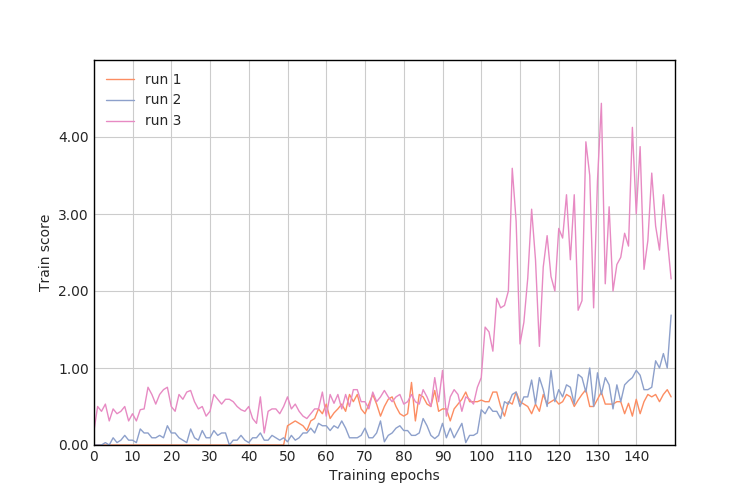
\includegraphics[width=0.9\columnwidth]{figures/freeway.png}
%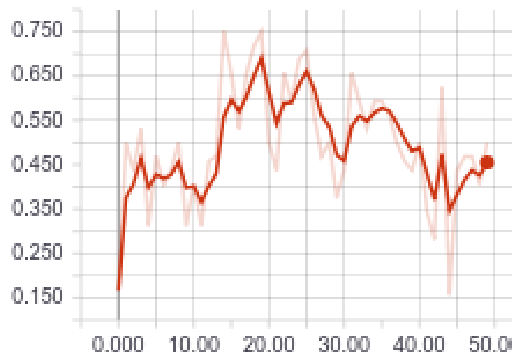
\includegraphics[width=1.8in]{figures/c0.png}
%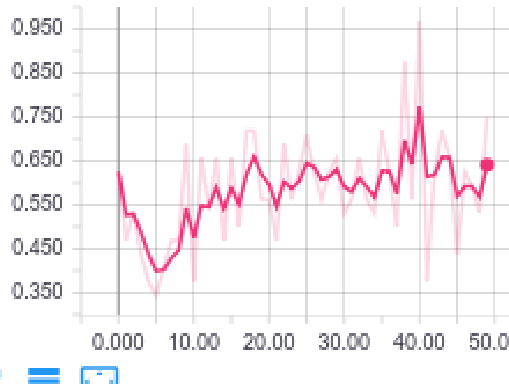
\includegraphics[width=1.8in]{figures/c1.png}
%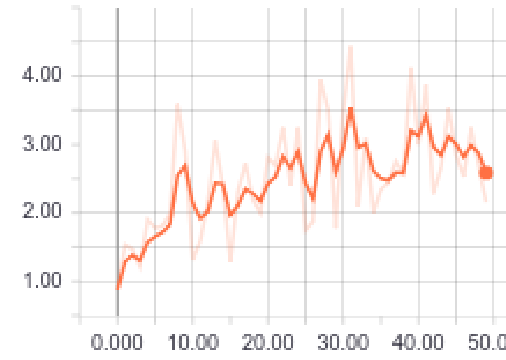
\includegraphics[width=1.8in]{figures/c3.png}
\caption{Three different runs of PPO training on simulated environment $env'$ for three iterations of the whole loop on \freeway\ training.
  The first iteration is epochs 0-50, the next 50-100 and the final one 100-150. Note that while all 3 models only reach scores below 4 in
  the shortened PPO training, all of them actually get scores above 10 when playing in the real environment, and the two better runs get above 20.
  Two of the runs already reach positive scores in the first iteration, while one run (orange) only reaches them in the second iteration -- this
  happens because no reward was seen in the first randomly generated data. In the third iteration the policies of the two runs that saw rewards
  in the first iteration get very good (scores above 20), while the third one learns slower.}
\label{fig:freeway_three_epochs}
\end{figure}

\paragraph{The accuracy metric on selected games.}\todo[inline]{(Henryk) @Piotr, I am assuming that you will fix it or remove}

\paragraph{Metrics}
We propose a new \textit{correct rewards predictions per sequence} metric to evaluate simulated environments. 
Let $t = (s, acs)$ be a tuple consisting of a state $s$ and a sequences of actions $acs$. We say that $env'$ is successful on $t$ if started from $s$ it produces the same total reward as the $env$ while executing subsequently actions $acs$.
Given $D$, a set of tuples as above we define \textit{correct rewards predictions per sequence} ratio on $D$ to be the ratio of successful $t$'s in $D$.
Typically, we evaluate simulated environment on $D$ with sequences $acs$ of a prescribed length $n\in \mathbb{N}$ generated according to some stochastically perturbed policy $\pi$. Intuitively, having good ratio in such a test means that the model behaves reliably in the neighborhood of $\pi$ in the time horizon $n$. %\todo{Piotr have a look here} %Thus, hopefully, it can be used in a reinforcement learning algorithm. 
We argue that this metric can correctly measure resemblance  of the simulated and original dynamics.  We believe it is better than the standard $L_2$ accuracy used in \cite{video_prediction,recurrent}, which has tendency to omit small but important objects (e.g. the ball in \pong).
\todo[inline]{So far we have one case: Pong, and number are very old, see Figure \ref{fig:correctness}}

\begin{figure}[H]
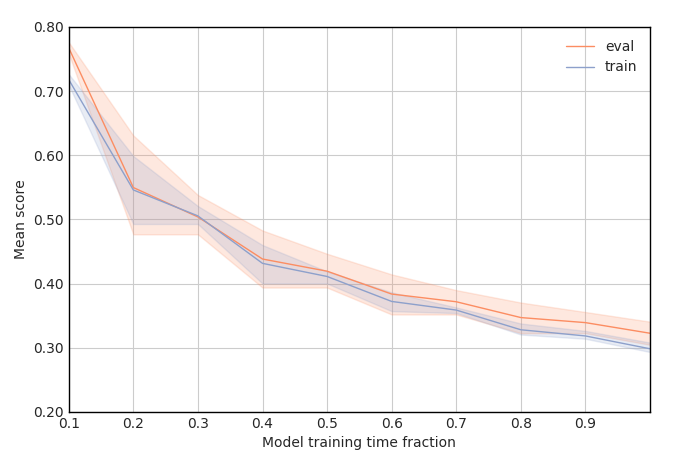
\includegraphics[width=0.35\textwidth]{figures/pong_ratio}%

\caption{Results on \pong: metric of correctness of rewards predictions per sequence.}
\label{fig:correctness}
\end{figure}

\paragraph{Analysis of the PPO modification}
\todo[inline]{So far we have one case: Pong, and number are very old, see Figure \ref{fig:ppo_mod}}

\begin{figure}[H]
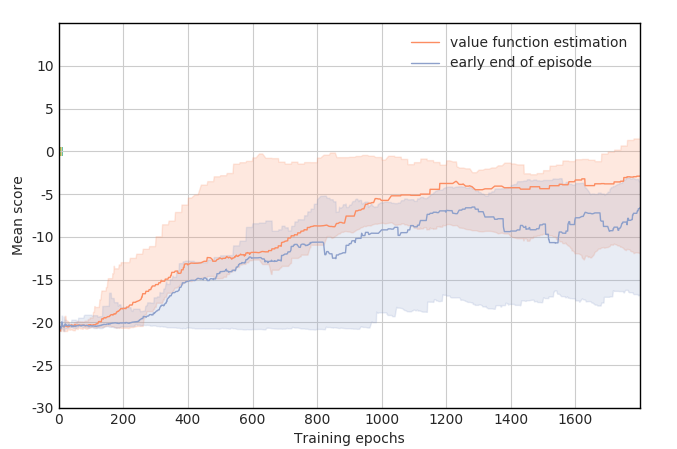
\includegraphics[width=0.35\textwidth]{figures/compare1000steps}
\caption{Results on \pong: a comparison of training in two settings: one assuming 0 reward at the end of simulated environment episode and improved version using value function estimation instead.}
\label{fig:ppo_mod}
\end{figure}